\documentclass{article}
\usepackage{epsfig,placeins}

%
% Copyright (C) 2007 Alan D. Brunelle <Alan.Brunelle@hp.com>
%
%  This program is free software; you can redistribute it and/or modify
%  it under the terms of the GNU General Public License as published by
%  the Free Software Foundation; either version 2 of the License, or
%  (at your option) any later version.
%
%  This program is distributed in the hope that it will be useful,
%  but WITHOUT ANY WARRANTY; without even the implied warranty of
%  MERCHANTABILITY or FITNESS FOR A PARTICULAR PURPOSE.  See the
%  GNU General Public License for more details.
%
%  You should have received a copy of the GNU General Public License
%  along with this program; if not, write to the Free Software
%  Foundation, Inc., 59 Temple Place, Suite 330, Boston, MA  02111-1307  USA
%
%  vi :set textwidth=75

\title{\texttt{btt} User Guide}
\author{Alan D. Brunelle (Alan.Brunelle@hp.com)}
\date{30 October 2008}

\begin{document}
\maketitle
%--------------
\section{\label{sec:intro}Introduction}

\texttt{btt} is a post-processing tool for the block layer IO tracing
tool called blktrace. As noted in its Users Guide, blktrace

  \begin{quotation}
    is a block layer IO tracing mechanism which provides detailed
    information about request queue operations up to user space.
  \end{quotation}

blktrace is capable of producing tremendous amounts of output in the
form of multiple individual traces per IO executed during the traced
run. It is also capable of producing some general statistics concerning
IO rates and the like. \texttt{btt} goes further and produces a variety
of overall statistics about each of the individual handling of IOs, and
provides data we believe is useful to plot to provide visual comparisons
for evaluation.

This document will discuss \texttt{btt} usage, provide some sample output,
and also show some interesting plots generated from the data provided
by the \texttt{btt} utility.

\bigskip
A short note on the ordering of this document -- the actual
command-line usage section occurs relatively late in the document (see
section~\ref{sec:cmd-line}), as we felt that discussing some of the
capabilities and output formats would make the parameter discussion
easier.

\bigskip
  This document refers to the output formats generated by \texttt{btt}
  version 2.00.  However, the descriptions are general enough to cover
  output formats prior to that.

\newpage\tableofcontents

\newpage\section{\label{sec:getting-started}Getting Started}

  The simple pipeline to get going with \texttt{btt} is to perform the
  following steps:

  \begin{enumerate}
    \item Run \texttt{blktrace}, specifying whatever devices and other
    parameters you want. You must save the traces to disk in this step,
    btt does not work in live mode.

    \item After tracing completes, run \texttt{blkrawverify}, specifying
    all devices that were traced (or at least on all devices that you
    will use \texttt{btt} with -- section~\ref{sec:o-D} shows how you
    can dictate which devices to use with btt). If blkrawverify finds
    errors in the trace streams saved, it is best to recapture the data
    -- utilizing \texttt{btt} on \emph{unclean} trace files produces
    inconsistent results.

    While this step is optional, we have found that performing this
    helps to ensure data coming from \texttt{btt} makes the most sense.

    \item Run \texttt{blkparse} with the \texttt{-d} option specifying
    a file to store the combined binary stream. (e.g.: \texttt{blkparse
    -d bp.bin ...}).

    \texttt{blktrace} produces a series of binary files
    containing parallel trace streams -- one file per CPU per
    device. \texttt{blkparse} provides the ability to combine all the
    files into one time-ordered stream of traces for all devices.

    \item Run \texttt{btt} specifying the file produced by
    \texttt{blkparse} utilizing the \texttt{-i} option (e.g.: \texttt{btt
    -i bp.bin ...}).

  \end{enumerate}

\newpage\section{\label{sec:output-overview}Output Overview}

  The major default areas of output provided by \texttt{btt}
  include\label{tl-defs}:

\begin{description}
  \item[average component times across all IOs] The time line of each IO
  is broken down into 3 major regions:

    \begin{enumerate}
      \item Time needed to insert or merge an incoming IO onto the request
      queue. This is the average time from when the IO enters the block
      IO layer (queue trace) until it is inserted (insert trace).

      This is denoted as \emph{Q2I} time.

      This is also broken down into two component times\footnote{On
      occasion there are also some time spent \emph{sleeping} waiting
      for a request. That occurs between the Q and G operations. You
      will see these listed as \texttt{S2G} times.}:

        \begin{description}
	  \item[Q2G] Time needed to \emph{get} a request (get request
	  trace).

	  \item[G2I] Time needed to put that request onto the request
	  queue (insert trace).
        \end{description}

      For \emph{merged} requests -- an incoming request that is merged
      with a previously submitted request -- we calculate \emph{Q2M}, the
      amount of time between the queue trace and the merge trace.

      \item Time spent on the request queue. The average time from when
      the IO is inserted or merged onto the request queue, until it is
      issued (issue trace) to the lower level driver.

      Referred to as \emph{I2D} time\footnote{The \emph{issue} trace
      is represented by a D in the blkparse output, hence its usage in
      btt to refer to issue traces. Note that an I is used to refer to
      \emph{insert} traces.}.

      \item Driver and device time -- the average time from when the
      actual IO was issued to the driver until is completed (completion
      trace) back to the block IO layer.

      This is referred to as the \emph{D2C} time\
    \end{enumerate}

  Two other sets of results are presented in this section:

    \begin{enumerate}
      \item \emph{Q2Q} which measures the time between queue traces
      in the system. This provides some idea as to how quickly IOs are
      being handed to the block IO layer.

      \item \emph{Q2C} which measures the times for the complete life cycle
      of IOs during the run\footnote{One of the areas that needs some
      work in \texttt{btt} is to better understand the multiplex nature of
      IOs during a run. In theory, one would like ${Q2I} + {I2D} + {D2C}
      = {Q2C}$ however, typically there are multiple queue traces that
      are combined via merges into a single IO issued and completed. We
      currently average the queue-to-insert and queue-to-merge times,
      and thus tend to be quite close to the expected equation.}

    \end{enumerate}

  For each row in this output, we provide a minimum, average, maximum
  (which are all presented in seconds), and overall count. As an
  example\footnote{As with this display, the author has taken some liberty
  in reformatting the output for better display on the printed page.}:

\begin{verbatim}
ALL            MIN           AVG           MAX           N
---- ------------- ------------- ------------- -----------
Q2Q    0.000000058   0.000012761   9.547941661     2262310
Q2I    0.000000272   0.000005995   0.104588839     2262311
I2D    0.000001446   0.094992714   0.239636864     2262311
D2C    0.000193721   0.030406554   1.634221408     2262311
Q2C    0.000207665   0.125405263   1.830917198     2262311
\end{verbatim}

  When tracking \emph{device mapper} devices, we also break down the
  \emph{Q2A} and \emph{Q2C} times for those IOs.

  \item[Device Overhead]

  Using the data from the previous chart, we can then provide some idea
  as to where IO spend most of the time on average. The following output
  shows the percentage of time spent in each of the phases of an
IO\footnote{It should be noted that incoming requests either go through:

\begin{enumerate}
  \item Q2G + Q2I

  or

  \item Q2M
\end{enumerate}
  before proceeding to I2D and D2C.}

\begin{verbatim}
       DEV |       Q2G       G2I       Q2M       I2D       D2C
---------- | --------- --------- --------- --------- ---------
 (  8, 80) |   0.0013%   0.0004%   0.0006%  88.5005%  11.4988%
---------- | --------- --------- --------- --------- ---------
   Overall |   0.0003%   0.0001%   0.0041%  21.4998%  78.4958%
\end{verbatim}

  \item[Device Merge Information]

  A key measurement when making changes in the system (software \emph{or}
  hardware) is to understand the block IO layer ends up merging incoming
  requests into fewer, but larger, IOs to the underlying driver. In this
  section, we show the number of incoming requests (Q), the number of
  issued requests (D) and the resultant ratio. We also provide values
  for the minimum, average and maximum IOs generated.

  Looking at the following example:

\begin{verbatim}
       DEV |      #Q    #D Ratio | BLKmin BLKavg BLKmax   Total
---------- | ------- ----- ----- | ------ ------ ------ -------
 ( 68, 64) | 2262311 18178 124.5 |      2    124    128 2262382
\end{verbatim}

  we see that (on average) the block IO layer is combining upwards of
  125 incoming requests into a single request down the IO stack. The
  resultant average IO size is 124 blocks.

  \item[Device Seek Information]

  Another useful measure is the variability in the sector distances
  between consecutively \emph{received -- queued} and \emph{submitted
  -- issued} IOs. The next two sections provides some rudimentary
  statistics to gauge the general nature of the sector differences
  between IOs. Values provided include the number of seeks (number of IOs
  submitted to lower level drivers), the \emph{mean} distance between
  IOs, the \emph{median} value for all seeks, and the \emph{mode} -
  the value(s) and the counts are provided for the latter.

  The first of the two sections displays values for Q2Q seek distances --
  providing a set of indicators showing how close incoming IO requests
  are to each other. The second section shows D2D seek distances --
  providing a set of indicators showing how close the IO requests are
  that are handled by underlying drivers.

\begin{verbatim}
      DEV | NSEEKS    MEAN MEDIAN | MODE
--------- | ------ ------- ------ | -------
( 68, 64) |  18178 19611.3      0 | 0(17522)
\end{verbatim}

  We have almost exclusively seen median and mode values of 0, indicating
  that seeks tend to have an equal amount of forward and backwards
  seeks. The larger the count for the mode in comparison to the total
  number of seeks is indicative as to how many IOs are coming out of
  the block IO layer in adjacent sectors. (Obviously, the higher this
  percentage, the better the underlying subsystems can handle them.)

  \item[Request Queue Plug Information]

  During normal operation, requests queues are \emph{plugged} and during
  such times the IO request queue elements are not able to be processed
  by underlying drivers. The next section shows how often the request
  queue was in such a state.

\begin{verbatim}
      DEV | # Plugs # Timer Us  | % Time Q Plugged
--------- | ------- ----------  | ----------------
( 68, 64) |     833(         0) |   0.356511895%
\end{verbatim}

  There are two major reasons why request queues are unplugged, and both
  are represented in the above table.

  \begin{enumerate}
    \item Explicit unplug request from some subsystem in the kernel.

    \item Timed unplugs, due to a request queue exceeding some temporal
    limit for being plugged.
  \end{enumerate}

  The total number of unplugs is equal to the number of plugs less the
  ones due to timer unplugs.

  \item[IOs per Unplug \& Unplugs-due-to-timeout]

  In this subsection one can see the average number of IOs on the request
  queue at the time of an unplug or unplug due to a timeout. The following
  sample shows a sample of both unplug sections:

\begin{verbatim}
==================== Plug Information ====================

       DEV |    # Plugs # Timer Us  | % Time Q Plugged
---------- | ---------- ----------  | ----------------
 (  8,  0) |       1171(       123) |   0.280946640%
 (  8, 32) |          4(         0) |   0.000325469%
---------- | ---------- ----------  | ----------------
   Overall |    # Plugs # Timer Us  | % Time Q Plugged
   Average |        587(        61) |   0.140636055%

       DEV |    IOs/Unp   IOs/Unp(to)
---------- | ----------   ----------
 (  8,  0) |        9.2          8.8
 (  8, 32) |        2.5          0.0
---------- | ----------   ----------
       DEV |    IOs/Unp   IOs/Unp(to)
   Overall |        9.2          8.8
\end{verbatim}

  This table and the preceding one have to be considered together --
  in the sample output in the immediately preceding table one can see
  how the larger number of data values for device (8,0) dominates in
  the overall average.

  \item[Active Requests At Q Information]

  An important consideration when analyzing block IO schedulers is to
  know how many requests the scheduler has to work with. The metric
  provided in this section details how many requests (on average) were
  being held by the IO scheduler when an incoming IO request was being
  handled. To determine this, \texttt{btt} keeps track of how many Q
  requests came in, and subtracts requests that have been issued (D).

  Here is a sample output of this sections:

\begin{verbatim}
==================== Active Requests At Q Information ====================

       DEV |  Avg Reqs @ Q
---------- | -------------
 ( 65, 80) |          12.0
 ( 65,240) |          16.9
...
 ( 66,112) |          44.2
---------- | -------------
   Overall | Avgs Reqs @ Q
   Average |          17.4
\end{verbatim}

\end{description}

\newpage
\subsection*{\label{sec:detailed-data}Detailed Data}

  In addition to the default sections output, if one supplies the
  \texttt{--all-data} or \texttt{-A} argument (see section~\ref{sec:o-A})
  to \texttt{btt} further sections are output:

\begin{description}
  \item[Per Process] As traces are emitted, they are tagged with the
  process ID of the currently running thread in the kernel. The process
  names are also preserved, and mapped to the ID. For each of the parts
  of the time line discussed above on page~\pageref{tl-defs}, a chart is
  provided which breaks down the traces according to process ID (name).

  One must be aware, however, that the process ID may not have anything
  to do with the originating IO. For example, if an application is
  doing buffered IO, then the actual submitted IOs will most likely
  come from some page buffer management daemon thread (like pdflush,
  or kjournald for example). Similarly, completion traces are rarely
  (if ever?) going to be associated with the process which submitted
  the IO in the first place.

  Here is a sample portion of this type of chart, showing Q2Q times
  per process:

\begin{verbatim}
          Q2Q         MIN         AVG         MAX       N
------------- ----------- ----------- ----------- -------
mkfs.ext3     0.000000778 0.000009074 1.797176188 1899371
mount         0.000000885 0.000672513 0.030638128      73
pdflush       0.000000790 0.000006752 0.247231307  179791
\end{verbatim}

  \item[Per Process Averages] The average columns from the above charts,
  are also presented in their own chart.

  \item[Per Device] Similar to the per-process display, \texttt{btt}
  will also break down the various parts of an IOs time line based upon a
  per-device criteria. Here's a portion of this area, displayed showing
  the issued to complete times (D2C).

\begin{verbatim}
      D2C         MIN         AVG         MAX      N
--------- ----------- ----------- ----------- ------
( 65, 80) 0.000140488 0.001076906 0.149739869 169112
( 65, 96) 0.000142762 0.001215221 0.173263182 155488
( 65,112) 0.000145221 0.001254966 0.124929936 165726
( 65,128) 0.000141896 0.001159596 0.775231052 169015
( 65,144) 0.000140832 0.001290985 0.211384698 210661
( 65,160) 0.000139915 0.001175554 0.073512063 133973
( 65,176) 0.000141254 0.001104870 0.073231310 145764
( 65,192) 0.000141453 0.001234460 0.167622507 140618
...
\end{verbatim}

  \item[Per Device Averages] The average columns from the above charts,
  are also presented in their own chart.

  \item[Q2D Histogram] A display of histogram buckets for the Q to D times
  -- basically, from where an IO enters the block IO layer for a given
  device, and when it is dispatched. The buckets are arranged via the
  time in seconds, as in:

\begin{verbatim}
==================== Q2D Histogram ====================

       DEV | <.005 <.010 <.025 <.050 <.075 <.100 <.250 <.500 < 1.0 >=1.0
 --------- | ===== ===== ===== ===== ===== ===== ===== ===== ===== =====
 ( 66, 80) |  61.2   7.9  12.1   7.9   3.0   1.4   1.5   0.2   0.0   4.6
 ( 65,192) |  42.3   5.0   8.7  30.0   8.9   3.0   1.8   0.1   0.0   0.1
 ( 65,128) |  34.3   5.3   8.9  32.0   9.7   3.7   5.3   0.6   0.0   0.1
...
 ( 65, 64) |  59.9   4.2   6.0  24.6   4.2   0.8   0.1   0.0   0.0   0.1
 ( 66, 64) |  62.6   8.1  12.7   7.9   2.4   0.6   0.1   0.0   0.0   5.4
========== | ===== ===== ===== ===== ===== ===== ===== ===== ===== =====
       AVG |  52.9   6.2  10.0  20.1   5.3   1.7   1.4   0.2   0.0   2.1
\end{verbatim}

\end{description}

\newpage\section{\label{sec:data-files}Data Files Output}

  Besides the averages output by default, the following 3 files are also
  created with data points which may be plotted.

\begin{description}
  \item[\emph{file}.dat] This file provides a notion of \emph{activity}
  for the system, devices and processes. The details of this file are
  provided in section~\ref{sec:activity}.

  \item[\emph{file}\_qhist.dat] Provides histogram data for the size of
  incoming IO requests, for more information see section~\ref{sec:qhist}.

  \item[\emph{file}\_dhist.dat] Provides histogram data for the size
  of IO requests submitted to lower layer drivers, for more information
  see section~\ref{sec:dhist}.

\end{description}

  In addition to the default data files output, there are optional data
  files which can be generated by btt. These include:

  \begin{description}
    \item[subset of \texttt{.avg} data, easily parsed ] When the
    \texttt{-X} option is specified \emph{and} the \texttt{-o} has also
    been specified, then a subset of the data produced by default is
    copied to another file that is \emph{more easily parsed.} Refer to
    section~\ref{sec:o-X} for full details.

    \item[iostat] iostat-like data can be distilled by btt, and is
    described in section~\ref{sec:iostat}.

    \item[per IO detail] Each and every IO traced can be output in a form
    that shows each of the IO components on consecutive lines (rather
    than grepping through a blkparse output file for example). The
    details on this file is included in section~\ref{sec:per-io}.

    \item[iostat] Latency information -- both Q2d, D2c and Q2C --
    on a per-IO basis can be generated. These are described in
    section~\ref{sec:lat}.

    \item[seek details] A set of data files containing all IO-to-IO
    sector differences can be output, with details found in
    section~\ref{sec:seek}.

    \item[unplug histogram details] A data file per device containing
    histogram output for the amount of IOs released at unplug time.
    Section~\ref{sec:o-u} has more details.
  \end{description}

\newpage\section{\label{sec:activity}Activity Data File}

  The activity data file contains a series of data values that indicate
  those periods of time when queue and complete traces are being
  processed.  The values happen to be in a format easily handled by
  xmgrace\footnote{\texttt{http://plasma-gate.weizmann.ac.il/Grace/}
  ``Grace is a WYSIWYG 2D plotting tool for the X Window System and
  M*tif.''}, but is easy to parse for other plotting and/or analysis
  programs.

  The file is split into pairs of sets of data points, where each pair
  contains a set of queue activity and a set of completion activity. The
  points are presented with the first column (X values) being the time
  (in seconds), and the second column (Y values) providing an on/off
  type of setting. For each pair, the Y values have two settings off
  (low) and on (high). For example, here is a snippet of a file showing
  some Q activity:

\begin{verbatim}
# Total System
#     Total System : q activity
0.000000000   0.0
0.000000000   0.4
0.000070381   0.4
0.000070381   0.0
1.023482637   0.0
1.023482637   0.4
6.998746618   0.4
6.998746618   0.0
7.103336799   0.0
7.103336799   0.4
17.235419786   0.4
17.235419786   0.0
26.783361447   0.0
26.783361447   0.4
26.832454929   0.4
26.832454929   0.0
28.870431266   0.0
28.870431266   0.4
28.870431266   0.4
28.870431266   0.0
\end{verbatim}

  What this indicates is that there was q activity for the system
  from 0.000000000 through 0.000070381, but was inactive from there to
  1.023482637, and so on. Section~\ref{sec:o-d} contains details on how
  to adjust btt's notion of what constitutes activity.

  The pairs are arranged as follows:

  \begin{itemize}
    \item First there is the total system activity -- meaning activity
    in either queue or completion traces across all devices.

    \item Next comes per-device activity information -- for each device
    being traced, that request queues Q and C traces are presented.

    \item Last we present pairs per-process.
  \end{itemize}

  Using this, one is then able to plot regions of activity versus
  inactivity -- and one can gather a sense of deltas between the queueing
  of IOs and when they are completed. Figure~\ref{fig:activity} shows
  a very simplistic chart showing some activity:

  \begin{figure}[hb]
  \leavevmode\centering
  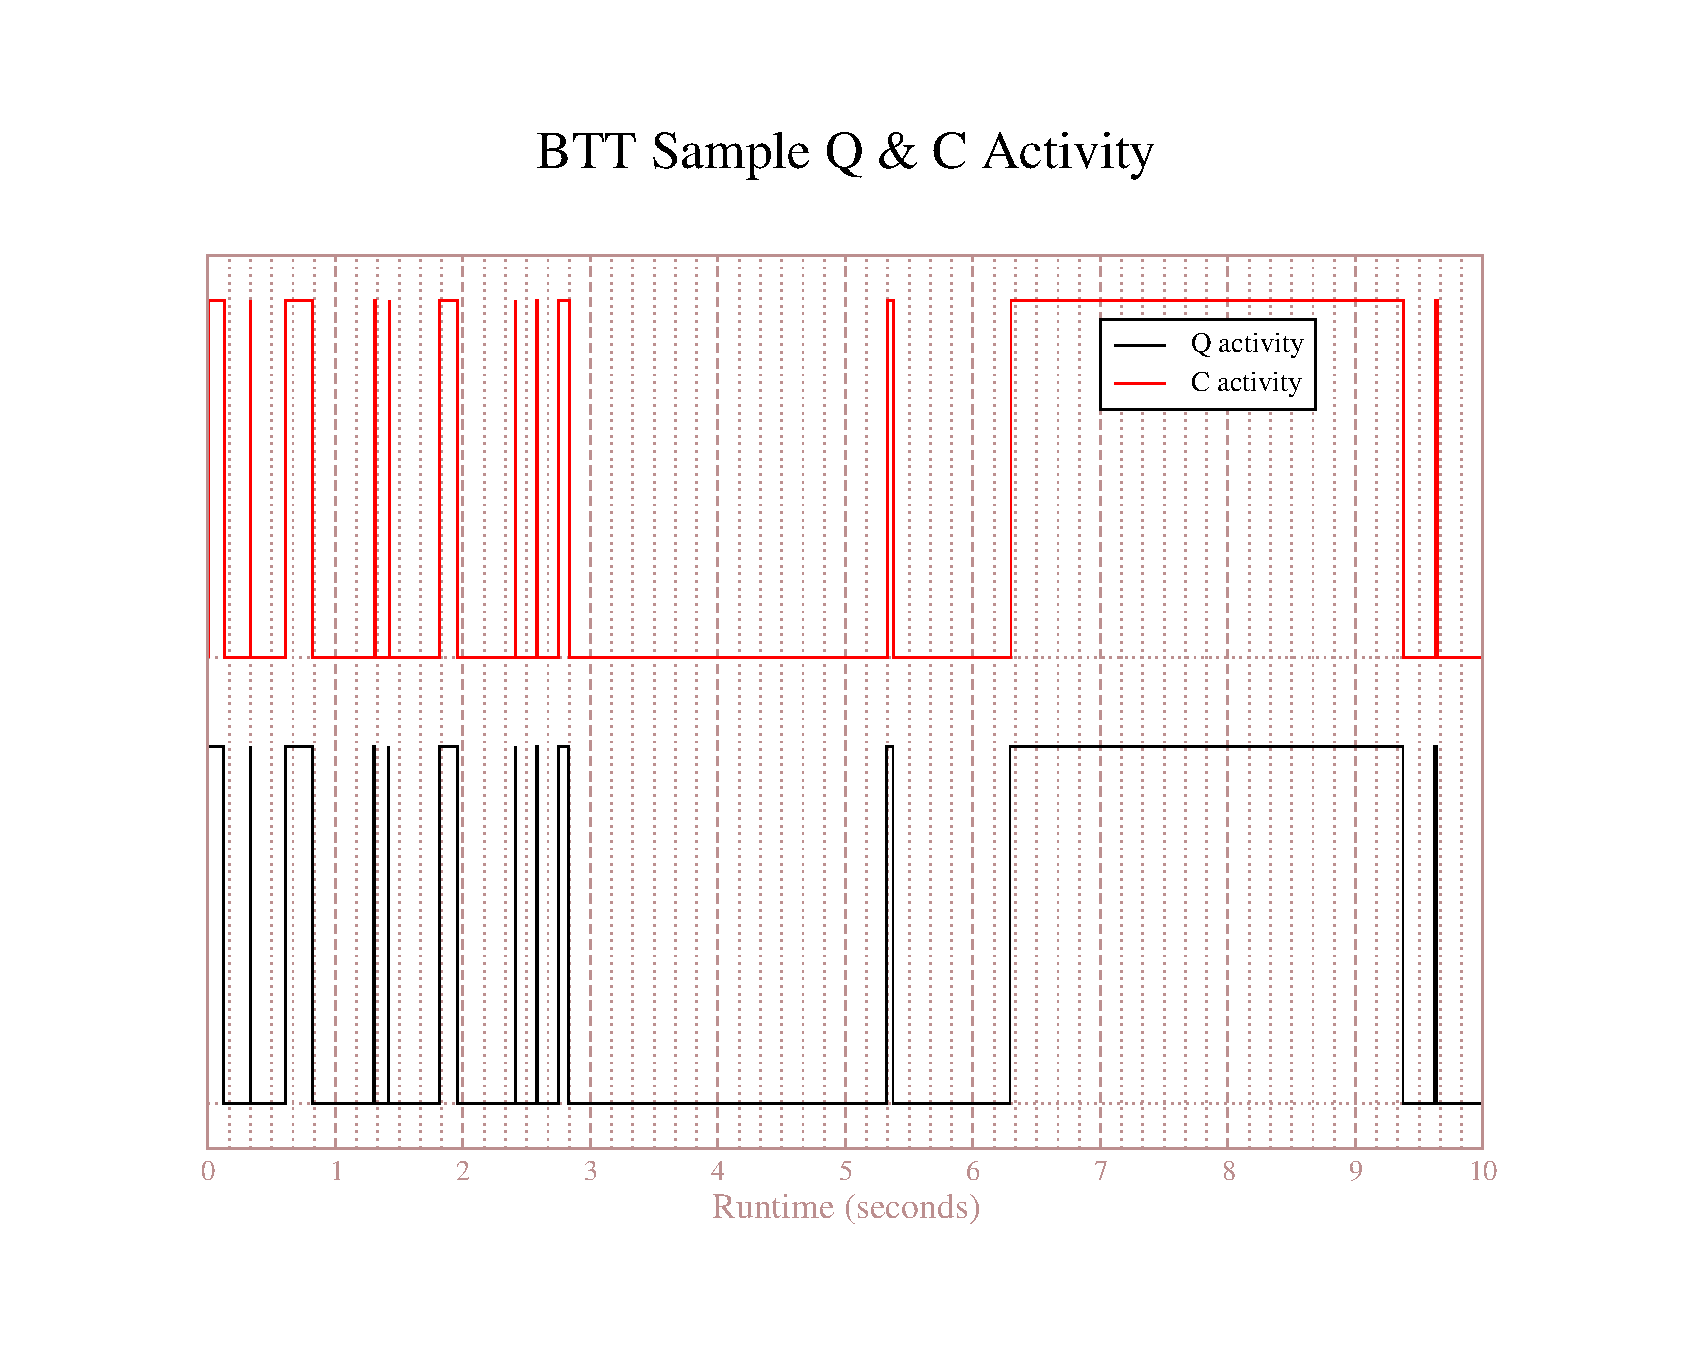
\epsfig{file=activity.eps,width=4.5in}
  \caption{\label{fig:activity}Simple Activity Chart}
  \end{figure}

  When the black line (system Q activity) is \emph{high}, then the system
  is seeing relatively continuous incoming queues. Conversely, when it is
  low, it represents an extended period of time where no queue requests
  were coming in. Similarly for the red line and C activity.

\newpage\section{\label{sec:hist}Histogram Data Files}

  The histogram data files provide information concerning incoming and
  outgoing IO sizes (in blocks). For simplicity, the histogram buckets
  are one-for-one for sizes up to 1,024 blocks in the IO, and then a
  single bucket for all sizes greater than or equal to 1,024 blocks.

  The files are again in grace-friendly format, with the first set
  containing data for the first 1,023 buckets, and a separate set
  representing sizes $\ge 1024$ blocks. (This is done so that one can
  easily use a separate formatting specification for the latter set.)

  The first column (X values) is the various IO sizes, and the second
  column (Y values) represents the number of IOs of that size.

\subsection*{\label{sec:qhist}Q Histogram Data File}

  Figure~\ref{fig:qhist} is a sample graph generated from data used during
  some real-world analysis\footnote{Note the logarithmic nature of the
  Y axis for this chart.}. With the visual representation provided by
  this, one can quickly discern some different characteristics between
  the 3 runs -- in particular, one can see that there is only a single
  red point (representing 8 blocks per IO), whereas the other two had
  multiple data points greater than 8 blocks.

  \begin{figure}[hb]
  \leavevmode\centering
  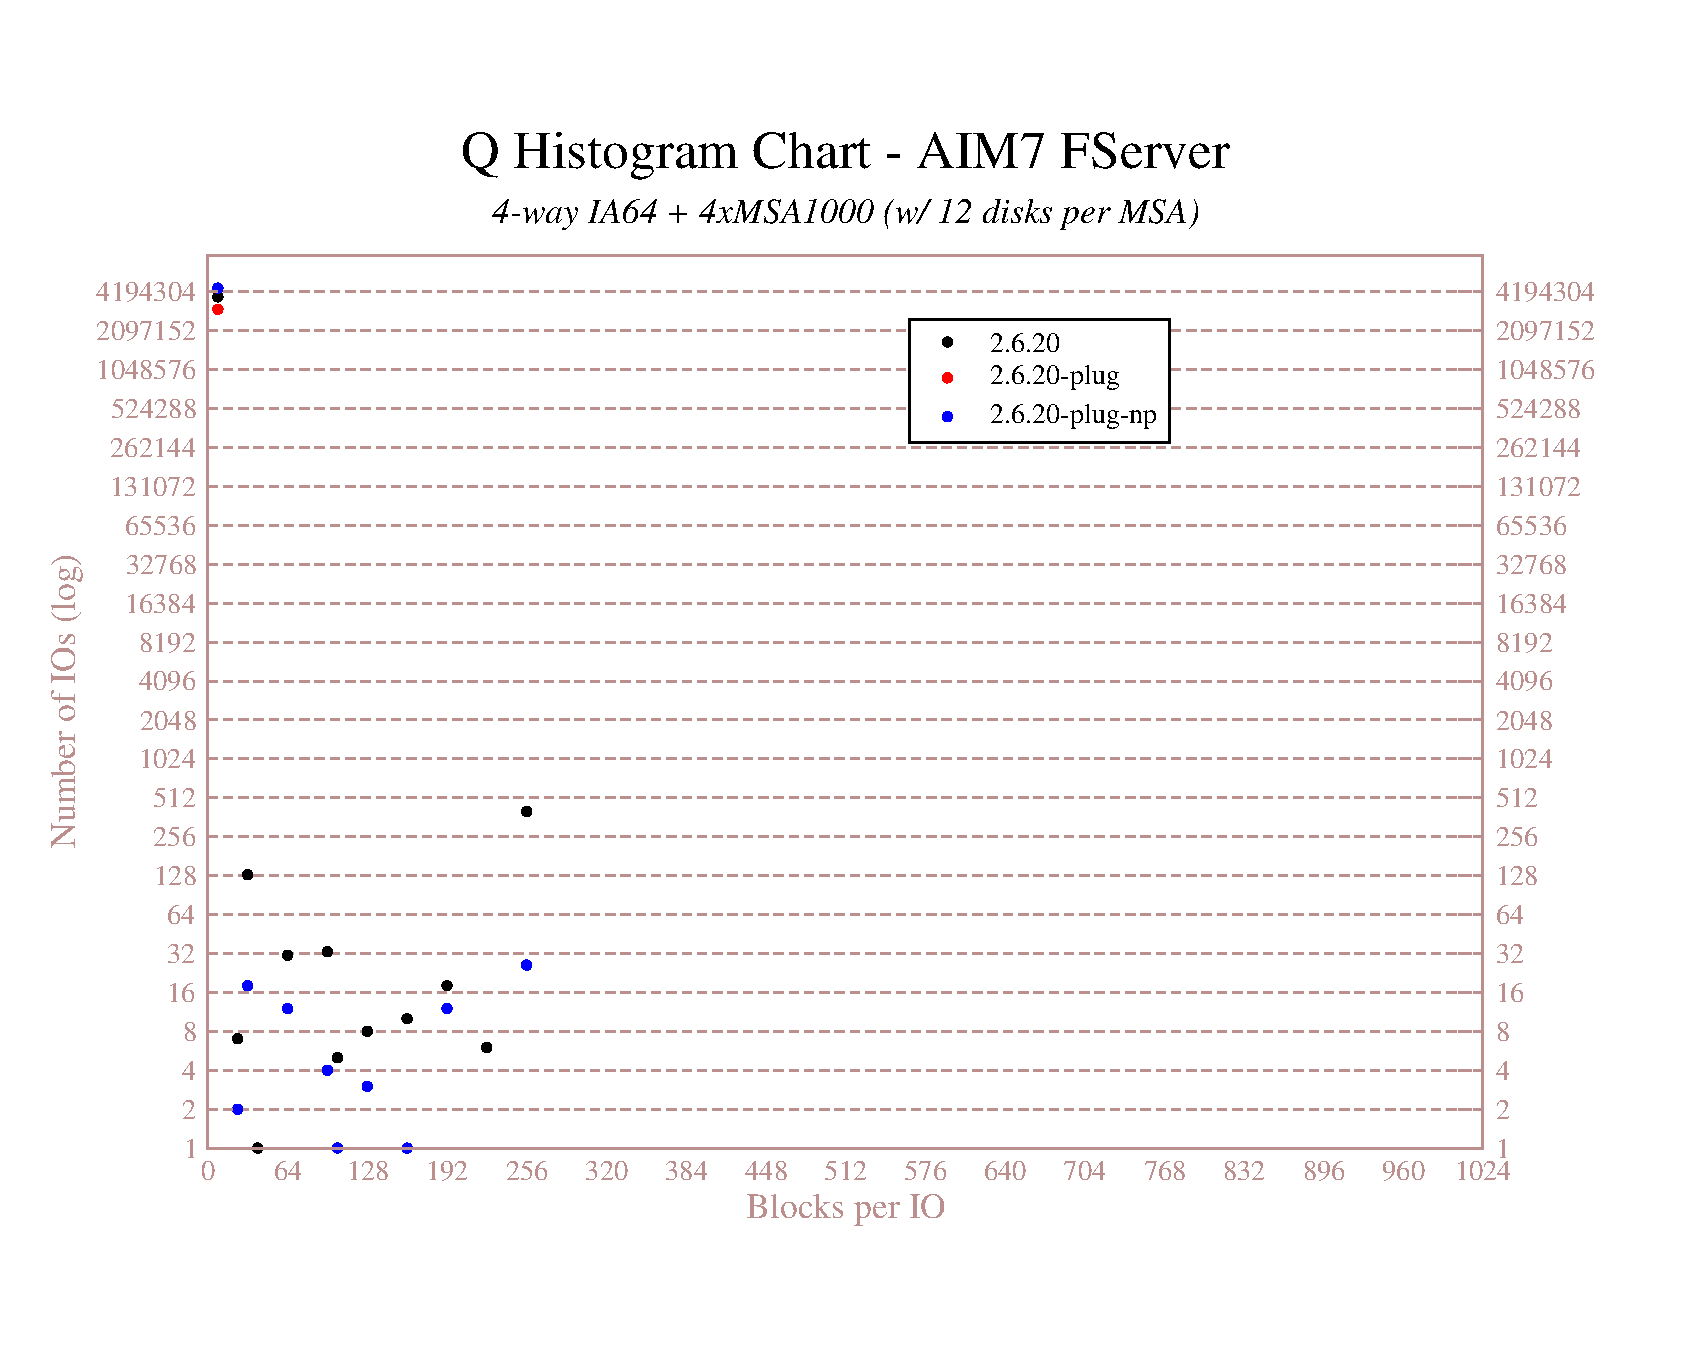
\epsfig{file=qhist.eps,width=4.5in}
  \caption{\label{fig:qhist}Q Histogram}
  \end{figure}

\subsection*{\label{sec:dhist}D Histogram Data File}

  Figure~\ref{fig:dhist} is a sample graph generated from data used during
  some real-world analysis\footnote{Note the logarithmic nature of the
  Y axis for this chart.}. Again, visually, one can see that the black
  and blue dots are somewhat similar below about 192 blocks per IO going
  out. And then one can make the broad generalization of higher reds,
  lower blues and blacks in the middle.

  \begin{figure}[hb]
  \leavevmode\centering
  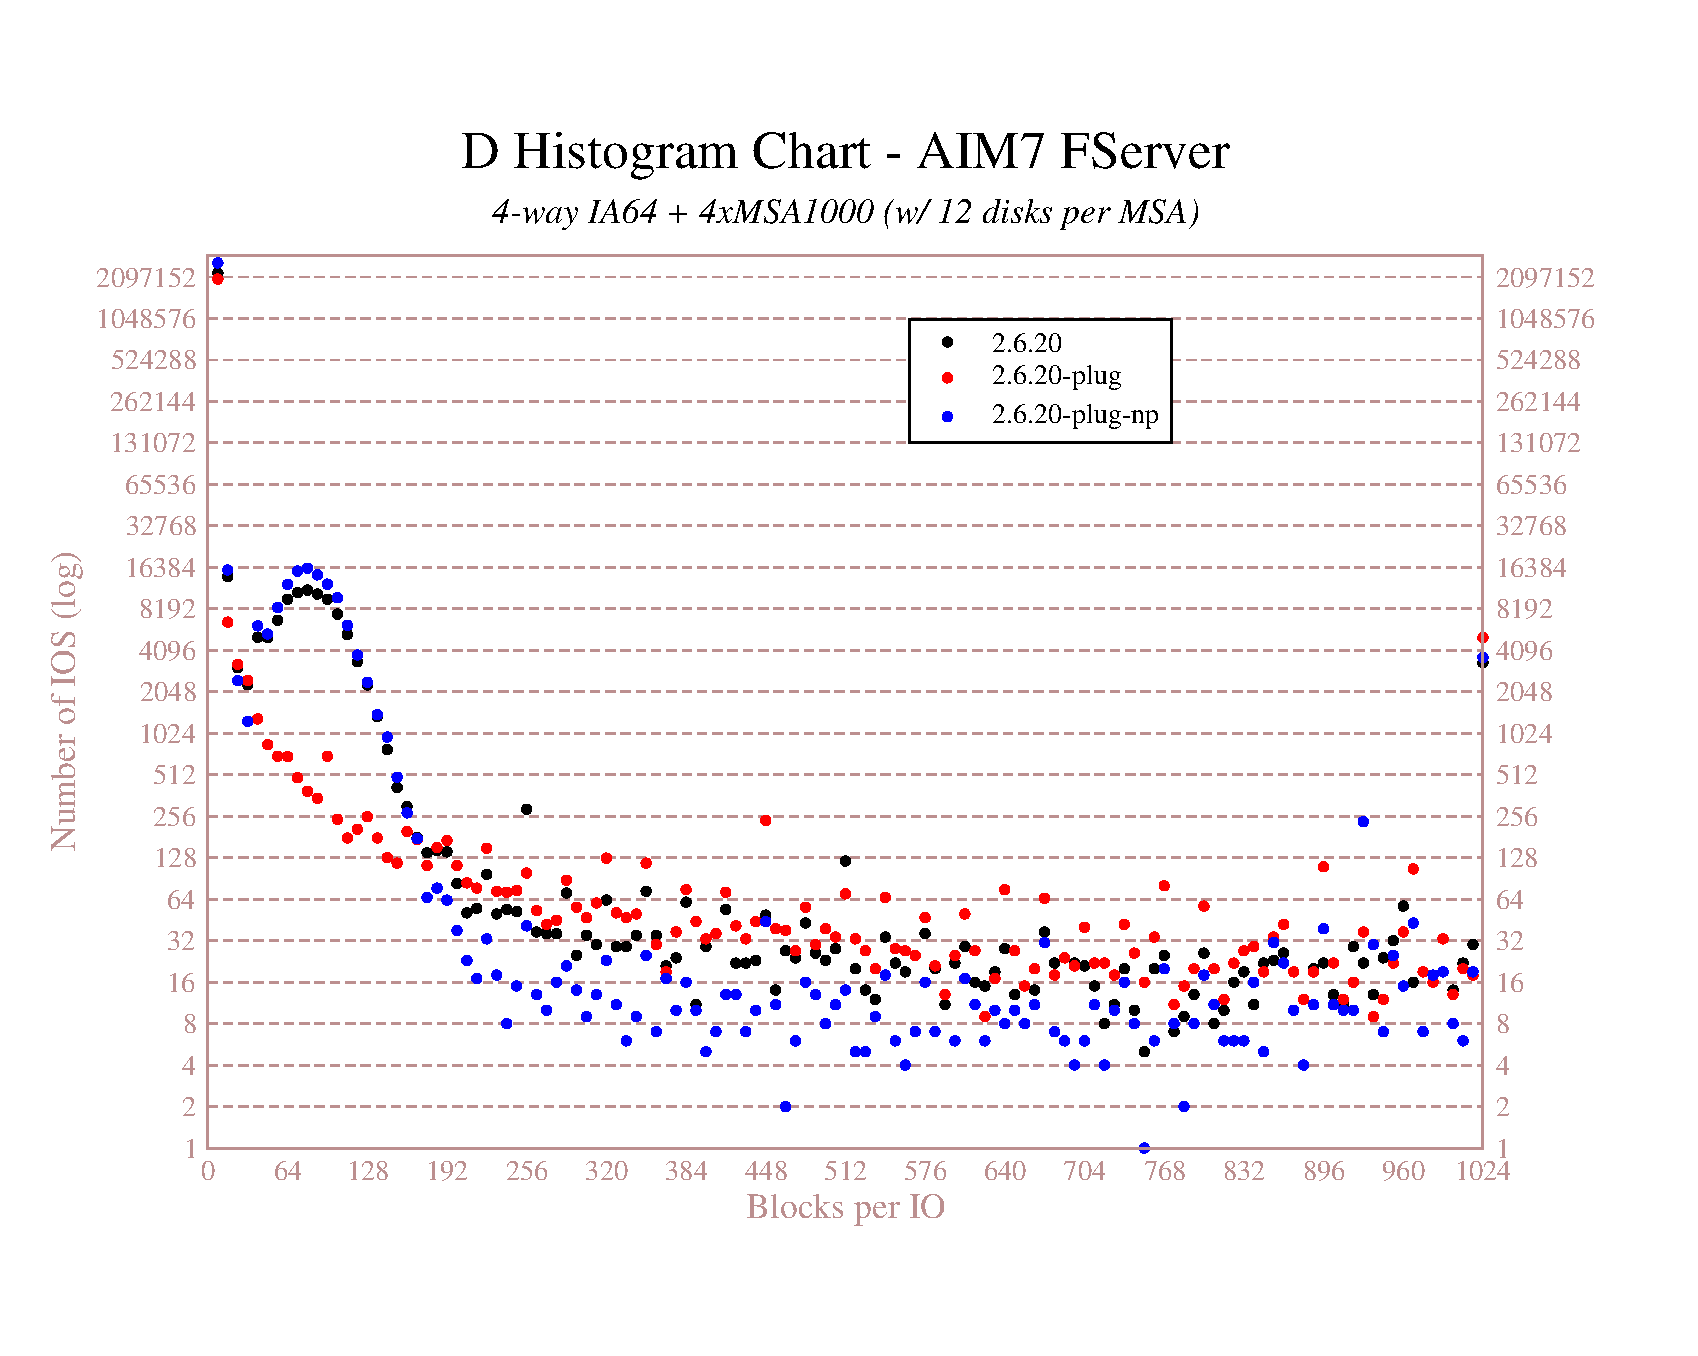
\epsfig{file=dhist.eps,width=4.5in}
  \caption{\label{fig:dhist}D Histogram}
  \end{figure}

\newpage\section{\label{sec:iostat}iostat Data File}
  \texttt{btt} attempts to produce the results from running an
  \texttt{iostat -x} command in parallel with the system as it is being
  traced. The fields (columns) generated by the \texttt{--iostat} or
  \texttt{-I} option can be seen from the following output snippet --
  note that the line has been split to fit on the printed page:

\begin{verbatim}
Device:       rrqm/s   wrqm/s     r/s     w/s    rsec/s    wsec/s
             rkB/s     wkB/s avgrq-sz avgqu-sz   await   svctm  %util   Stamp
...
(  8, 16)       0.00     0.00    0.00 1005.30      0.00 152806.36     
              0.00  76403.18   152.00    31.00    0.00    0.00   0.00   71.79
...
(  8, 16)       1.02     5.80    0.34    1.07      4.03     55.62
              2.02     27.81    42.13     0.61    0.00   21.90   0.00   TOTAL
\end{verbatim}

  Note that the STAMP field contains the runtime (in seconds) for that
  line of data.

\newpage\section{\label{sec:per-io}Per-IO Data File}

  \texttt{btt} can produce a text file containing time line data for each
  IO processed. The time line data contains rudimentary information for
  the following stages:

  \begin{itemize}
    \item queue traces
    \item get request traces
    \item insert traces
    \item merge traces
    \item issue traces
    \item completion traces
    \item remap traces
  \end{itemize}

  The \emph{--per-io-dump} or \emph{-p} option triggers this behavior,
  and will produce a file containing streams of IOs (separated by blank
  spaces). As an example, here is a snippet of 4 IOs that were merged
  together, you will note there are 3 merged IOs, and 1 inserted in the
  stream. The issue and completion traces are replicated per IO.

\begin{verbatim}
 66,0  :     0.763283556 Q       6208+8  
             0.763300157 I       6208+8  
             0.763296365 G       6208+8  
             0.763338848 D       6208+32 
             0.763705760 C       6208+32 

 66,0  :     0.763314550 Q       6224+8  
             0.763315341 M       6224+8  
             0.763338848 D       6208+32 
             0.763705760 C       6208+32 

 66,0  :     0.763321010 Q       6232+8  
             0.763321775 M       6232+8  
             0.763338848 D       6208+32 
             0.763705760 C       6208+32 

 65,240:     0.763244173 Q       6216+8  
             0.763244974 M       6216+8  
             0.763374288 D       6208+32 
             0.763826610 C       6208+32 
\end{verbatim}

  The columns provide the following information:

  \begin{enumerate}
    \item Device major/minor.

    \item Time of the trace (seconds from the start of the run)

    \item Trace type

    \item start block + number of blocks
  \end{enumerate}
 
\newpage\section{\label{sec:lat}\label{sec:lat-q2d}\label{sec:lat-q2c}\label{sec:lat-d2c}Latency Data Files}

  The latency data files which can be optionally produced by \texttt{btt}
  provide per-IO latency information, one for queue time (Q2D), one
  for total IO time (Q2C) and one for latencies induced by lower layer
  drivers and devices (D2C).

  In both cases, the first column (X values) represent runtime (seconds),
  while the second column (Y values) shows the actual latency for a
  command at that time (either Q2D, D2C or Q2C).

\newpage\section{\label{sec:seek}Seek Data Files}

  \texttt{btt} can also produce two data files containing all IO-to-IO sector
  deltas, providing seek information which can then be plotted. The
  produced data file contains 3 sets of data:

  \begin{enumerate}
     \item Combined data -- all read and write IOs

     \item Read data -- just seek deltas for reads

     \item Write data -- just seek deltas for writes
  \end{enumerate}

  The format of the output file names is to have the name generated by
  the following fields separated by underscores (\texttt{\_}):
 
  \begin{itemize}
    \item The prefix provided as the argument to the \texttt{-s} option.
    \item The major and minor numbers of the device separated by a comma.
    \item The string \texttt{q2q} or \texttt{d2d}, indicating the Q2Q or
          D2D seeks, respectively.
    \item One of the following characters:
    	\begin{description}
	  \item[r] For read (device to system) IOs
	  \item[w] For write (system to device) IOs
	  \item[c] Combined -- both read and write IOs
	\end{description}
  \end{itemize}

  An example name would be after specifying \texttt{-s seek} would be:
  \texttt{seek\_065,048\_q2q\_w.dat}.

  The format of the data is to have the runtime values (seconds since
  the start of the run) in column 1 (X values); and the difference in
  sectors from the previous IO in column 2 (Y values). Here is a snippet
  of the first few items from a file:

\begin{verbatim}
# Combined
     0.000034733           35283790.0
     0.000106453           35283790.0
     0.005239009           35283950.0
     0.006968575           35283886.0
     0.007218709           35283694.0
     0.012145393           35283566.0
     0.014980835          -35848914.0
     0.024239323          -35848914.0
     0.024249402          -35848914.0
     0.025707095          -35849072.0
     ...
\end{verbatim}

  Figure~\ref{fig:seek} shows a simple graph that can be produced which
  provides visual details concerning seek patterns.

  \begin{figure}[h!]
  \leavevmode\centering
  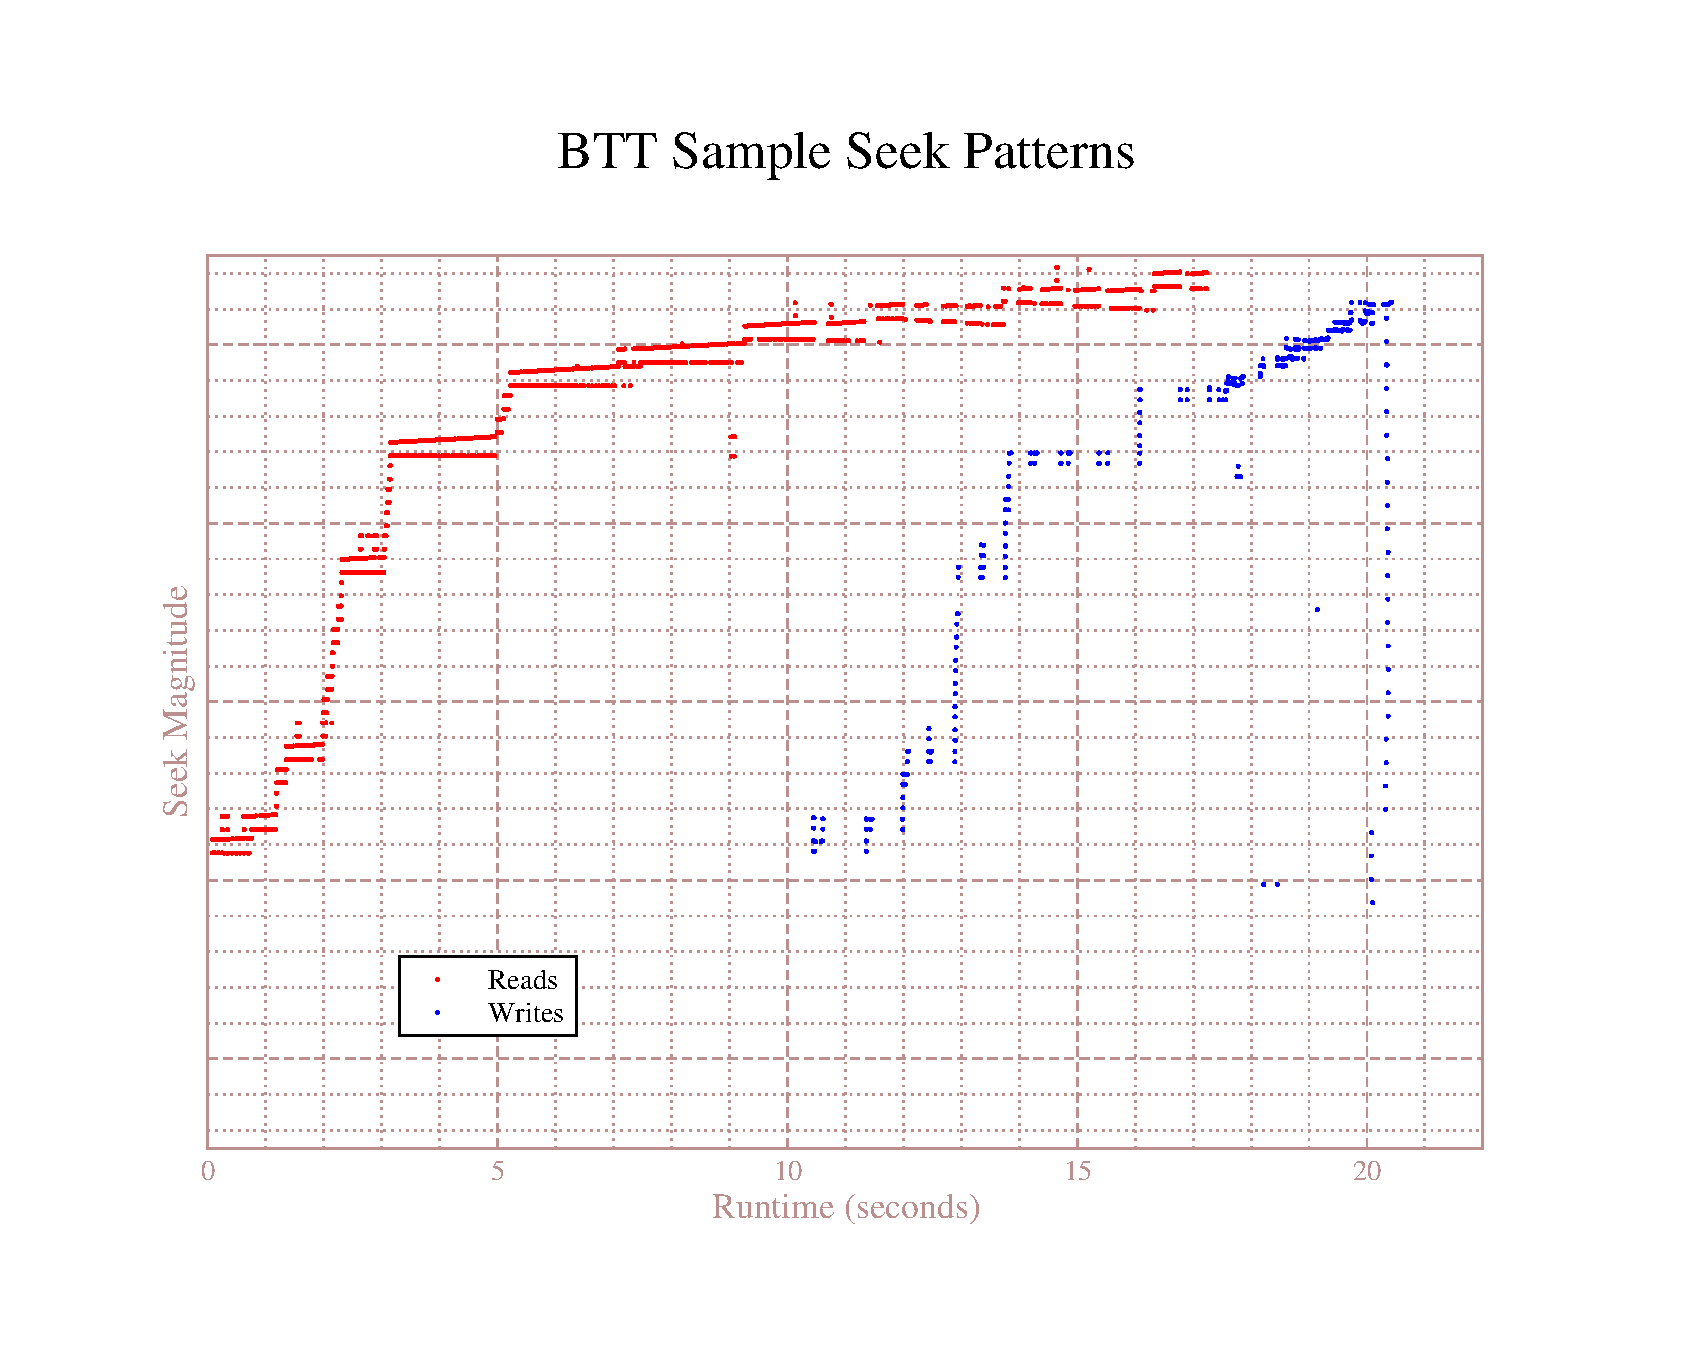
\epsfig{file=seek.eps,width=4.5in}
  \caption{\label{fig:seek}Seek Chart}
  \end{figure}
  \FloatBarrier

  The seek difference is calculated in one of two ways:

  \begin{description}
    \item[default] By default, the seek distance is calculated as the
    \emph{closest} distance between the previous IO and this IO. The
    concept of \emph{closeness} means that it could either be the
    \emph{end} of the previous IO and the beginning of the next, or the
    end of this IO and the start of the next.

    \item[\texttt{-a}] If the \texttt{-a} or \texttt{--seek-absolute}
    option is specified, then the seek distance is simply the difference
    between the end of the previous IO and the start of this IO.
  \end{description}

\newpage\subsection{\label{sec:sps-spec}Seeks Per Second}

  When the \texttt{-m} option provides a name, Q2Q and/or D2D seeks
  will trigger \texttt{btt} to output seeks-per-second information. The
  first column will contain a time value (seconds), and the second column
  will indicate the number of seeks per second at that point.

  When there is only a single data point within a 1-second window,
  \texttt{btt} will just output the time value for the point, and the
  value 1.0 in the second column. If there is no perceived difference
  in the times present for the current sample, then the second columns
  value is the number of seeks present at that time.

  Otherwise, if $\alpha$ and $\Omega$ are the first and last times
  seen within a 1-second window, and $\nu$ are the number of seeks seen
  in that time frame, then:

  \begin{description}
    \item[column 1] Midway point in time for this span, or: \hfill$\alpha +
    {{(\Omega - \alpha)} / 2}$

    \item[column 2] Average seeks per second over this span, or: \hfill$\nu  /
    {(\Omega - \alpha)}$
  \end{description}

  Figure~\ref{fig:sps} shows a simple pair of graphs generated from
  \texttt{-m} output:

  \begin{figure}[h!]
  \leavevmode\centering
  \epsfig{file=sps.eps,width=4.5in}
  \caption{\label{fig:sps}Seeks-per-second Chart}
  \end{figure}
  \FloatBarrier

\newpage\section{\label{sec:cmd-line}Command Line}

\begin{verbatim}
Usage: btt 2.06
[ -a               | --seek-absolute ]
[ -A               | --all-data ]
[ -B <output name> | --dump-blocknos=<output name> ]
[ -d <seconds>     | --range-delta=<seconds> ]
[ -D <dev;...>     | --devices=<dev;...> ]
[ -e <exe,...>     | --exes=<exe,...>  ]
[ -h               | --help ]
[ -i <input name>  | --input-file=<input name> ]
[ -I <output name> | --iostat=<output name> ]
[ -l <output name> | --d2c-latencies=<output name> ]
[ -L <freq>        | --periodic-latencies=<freq> ]
[ -m <output name> | --seeks-per-second=<output name> ]
[ -M <dev map>     | --dev-maps=<dev map>
[ -o <output name> | --output-file=<output name> ]
[ -p <output name> | --per-io-dump=<output name> ]
[ -q <output name> | --q2c-latencies=<output name> ]
[ -Q <output name> | --active-queue-depth=<output name> ]
[ -s <output name> | --seeks=<output name> ]
[ -S <interval>    | --iostat-interval=<interval> ]
[ -t <sec>         | --time-start=<sec> ]
[ -T <sec>         | --time-end=<sec> ]
[ -u <output name> | --unplug-hist=<output name> ]
[ -V               | --version ]
[ -v               | --verbose ]
[ -X               | --easy-parse-avgs ]
[ -z <output name> | --q2d-latencies=<output name> ]
\end{verbatim}

\subsection{\label{sec:o-a}\texttt{--seek-absolute}/\texttt{-a}}

  When specified on the command line, this directs btt to calculate
  seek distances based solely upon the ending block address of one IO,
  and the start of the next.  By default \texttt{btt} uses the concept
  of the closeness to either the beginning or end of the previous IO. See
  section~\ref{sec:seek} for more details about seek distances.

\subsection{\label{sec:o-A}\texttt{--all-data}/\texttt{-A}}

  Normally \texttt{btt} will not print out verbose information
  concerning per-process and per-device data (as outlined in
  section~\ref{sec:detailed-data}). If you desire that level of
  detail you can specify this option.

\subsection{\label{sec:o-B}\texttt{--dump-blocknos}/\texttt{-B}}

  This option will output absolute block numbers to three files prefixed
  by the specified output name:

  \begin{description}
    \item[\emph{prefix}\_\emph{device}\_r.dat] All read block numbers are
    output, first column is time (seconds), second is the block number,
    and the third column is the ending block number.

    \item[\emph{prefix}\_\emph{device}\_w.dat] All write block numbers are
    output, first column is time (seconds), second is the block number,
    and the third column is the ending block number.

    \item[\emph{prefix}\_\emph{device}\_c.dat] All block numbers (read
    and write) are output, first column is time (seconds), second is
    the block number, and the third column is the ending block number.
  \end{description}

\subsection{\label{sec:o-d}\texttt{--range-delta}/\texttt{-d}}

  Section~\ref{sec:activity} discussed how \texttt{btt} outputs a file
  containing Q and C activity, the notion of \emph{active} traces simply
  means that there are Q or C traces occurring within a certain period
  of each other. The default values is 0.1 seconds; with this option
  allowing one to change that granularity. The smaller the value, the
  more data points provided.

\subsection{\label{sec:o-D}\texttt{--devices}/\texttt{-D}}

  Normally, \texttt{btt} will produce data for all devices detected in
  the traces parsed. With this option, one can reduce the analysis to
  one or more devices provided in the string passed to this option. The
  device identifiers are the major and minor number of each device, and
  each device identifier is separated by a colon (:). A valid specifier
  for devices 8,0 and 8,8 would then be: \texttt{"8,0:8,8"}.

\subsection{\label{sec:o-e}\texttt{--exes}/\texttt{-e}}

  Likewise, \texttt{btt} will produce data for all processes (executables)
  found in the traces. With this option, one can specify which processes
  you want displayed in the output. The format of the string passed is
  a list of executable \emph{names} separated by commas (,). An example
  would be \texttt{"-e mkfs.ext3,mount"}.

\subsection{\label{sec:o-h}\texttt{--help}/\texttt{-h}}

  Prints out the simple help information, as seen at the top of
  section~\ref{sec:cmd-line}.

\subsection{\label{sec:o-i}\texttt{--input-file}/\texttt{-i}}

  Specifies the binary input file that \texttt{btt} will interpret traces
  in. See section~\ref{sec:getting-started} for information concerning
  binary trace files.

\subsection{\label{sec:o-I}\texttt{--iostat}/\texttt{-I}}

  This option triggers \texttt{btt} to generate iostat-like output to the
  file specified. Refer to section~\ref{sec:iostat} for more information
  on the output produced.

\subsection{\label{sec:o-l}\texttt{--d2c-latencies}/\texttt{-l}}

  This option instructs \texttt{btt} to generate the D2C latency file
  discussed in section~\ref{sec:lat-d2c}.

\subsection{\label{sec:o-L}\texttt{--periodic-latencies}/\texttt{-L}}

  When given a value greater than 0, this option will create two data
  files (q2c \& d2c) per device containing a periodic timestamp \&
  average latency over that period.

\subsection{\label{sec:o-m}\texttt{--seeks-per-second}\texttt{-m}}

  Tells \texttt{btt} to output seeks per second information.  Each device
  being measured can have up to 2 files output: One with Q2Q information
  and one with D2D seek information. Information on the output produced
  can be found in section~\ref{sec:sps-spec}.

  \begin{quote}
    \textbf{Note: This requires seek output to be selected -- see
    section~\ref{sec:seek}.}
  \end{quote}

\subsection{\label{sec:o-M}\texttt{--dev-maps}/\texttt{-M}}

  Internal option, still under construction.

\subsection{\label{sec:o-o}\texttt{--output-file}/\texttt{-o}}

  Normally \texttt{btt} sends the statistical output (covered in
  section~\ref{sec:output-overview}) to standard out, if you specify
  this option this data is redirected to the file specified.

\subsection{\label{sec:o-p}\texttt{--per-io-dump}/\texttt{-p}}

  This option tells \texttt{btt} to generate the per IO dump file as
  discussed in section~\ref{sec:per-io}.

\subsection{\label{sec:o-q}\texttt{--q2c-latencies}/\texttt{-q}}

  This option instructs \texttt{btt} to generate the Q2C latency file
  discussed in section~\ref{sec:lat-q2c}.

\subsection{\label{sec:o-Q}\texttt{--active-queue-depth}/\texttt{-Q}}

  This option tells \texttt{btt} to generate a data file (using the given
  name as a base) which contains: A time stamp in the first column,
  and then the number of \emph{active} requests issued to the device
  driver. (The value is incremented when an \emph{issue} is performend,
  and decremented when a \emph{complete} is performed.

\subsection{\label{sec:o-s}\texttt{--seeks}/\texttt{-s}}

  This option instructs \texttt{btt} to generate the seek data file
  discussed in section~\ref{sec:seek}.

\subsection{\label{sec:o-S}\texttt{--iostat-interval}/\texttt{-S}}

  The normal \texttt{iostat} command allows one to specify the snapshot
  interval, likewise, \texttt{btt} allows one to specify how many seconds
  between its generation of snapshots of the data via this option. Details
  about the iostat-like capabilities of \texttt{btt} may be found in
  section~\ref{sec:iostat}.

\subsection{\label{sec:o-tT}\texttt{--time-start}/\texttt{-t} and
\texttt{--time-end}/\texttt{T}}

  \begin{quote}
    \emph{This \texttt{btt} capability is still under construction, results are
    not always consistent at this point in time.}
  \end{quote}

  These options allow one to dictate to \texttt{btt} when to start and stop
  parsing of trace data in terms of seconds since the start of the run. The
  trace chosen will be between the start time (or 0.0 if not
  specified) and end time (or the end of the run) specified.

\subsection{\label{sec:o-u}\texttt{--unplug-hist}/\texttt{-u}}

  This option instructs \texttt{btt} to generate a data file containing
  histogram information for \emph{unplug} traces on a per device
  basis. It shows how many times an unplug was hit with a specified
  number of IOs released. There are 21 output values into the file, as
  follows:

  \medskip
  \begin{tabular}{ll}
\textbf{X value} & \textbf{Representing Counts} \\\hline
0 & 0\dots\/4 \\
1 & 5\dots\/9 \\
2 & 10\dots\/14 \\
\dots & \dots\dots\\
19 & 95\dots\/99 \\
20 & 100+ \\
  \end{tabular}

  \medskip
  The file name(s) generated use the text string passed as an argument for
  the prefix, followed by the device identifier in \texttt{major,minor}
  form, with a \texttt{.dat} extension (as an example, with \texttt{-u
  up\_hist} specified on the command line: \texttt{up\_hist\_008,032.dat}.

\subsection{\label{sec:o-V}\texttt{--version}/\texttt{-V}}

  Prints out the \texttt{btt} version, and exits.

\subsection{\label{sec:o-v}\texttt{--verbose}/\texttt{-v}}

  While \texttt{btt} is processing data, it will put out periodic (1-second
  granularity) values describing the progress it is making through the
  input trace stream. The value describes how many traces have been
  processed. At the end of the run, the overall number of traces, trace
  rate (number of thousands of traces per second), and the real time for
  trace processing and output are displayed. Example (note: the interim
  trace counts are put out with carriage returns, hence, they overwrite
  each time):

\begin{verbatim}
# btt -i bp.bin -o btt -v
Sending range data to bttX.dat
Sending stats data to bttX.avg
 287857 t
1414173 t
1691581 t
...
4581291 traces @ 279.7 Ktps
16.379036+0.000005=16.379041
\end{verbatim}

\subsection{\label{sec:o-X}\texttt{--easy-parse-avgs}/\texttt{-X}}

  \emph{Some} of the data produced by default can also be shipped
  simultaneously to another file in an easy to parse form. When
  the \texttt{-o} option is selected (thus producing a file with a
  \texttt{.avg} exentsion), \emph{and} the \texttt{-X} flag is present,
  then \texttt{btt} will generate this file.

  The format is space-delimited values starting with a 3-character
  \emph{record} indicator, then the device information (either major,minor
  or the device name when \texttt{-M} is specified), and then a number of
  fields representing data values. The following table shows the record
  identifiers and the fields provided:

  \bigskip
  \begin{tabular}{|l|l|}\hline
  \textbf{Record} & \textbf{Description}\\\hline
  \texttt{DMI}	& Device Merge Information:\\
		& \#Q \#D Ratio BLKmin BLKavg BLKmax Total\\\hline
  \texttt{QSK}	& Device Q2Q Seek Information:\\
		& NSEEKS MEAN MEDIAN MODE N-MODE mode\ldots\\\hline
  \texttt{DSK}	& Device D2D Seek Information:\\
		& NSEEKS MEAN MEDIAN MODE N-MODE mode\ldots\\\hline
  \texttt{PLG}	& Plug Information:\\
		& \#Plugs \#TimerUnplugs \%TimeQPlugged\\\hline
  \texttt{UPG}	& Unplug Information:\\
		& IOsPerUnplug IOsPerUnplugTimeout\\\hline
  \texttt{ARQ}	& Active Requests at Q Information:\\
  		& AvgReqs@Q\\\hline\hline
  \texttt{Q2Q}  & Queue-to-Queue times:\\
  \texttt{Q2G}  & Queue-to-GetRequest times:\\
  \texttt{S2G}  & Sleep-to-GetRequest times:\\
  \texttt{G2I}  & GetRequest-to-Insert times:\\
  \texttt{Q2M}  & Queue-to-Merge times:\\
  \texttt{I2D}  & Insert-to-Issue times:\\
  \texttt{M2D}  & Merge-to-Issue times:\\
  \texttt{D2C}  & Issue-to-Complete times:\\
  \texttt{Q2C}  & Queue-to-Complete times:\\
                & MIN AVG MAX N\\\hline
  \end{tabular}

  \bigskip
  A sample output file would look like:

  \begin{verbatim}
Q2Q 0.000000001 0.003511356 9.700000000 309906
Q2G 0.000000001 0.774586535 805.300000000 106732
S2G 0.000000001 0.072525952 0.370000000 578
G2I 0.000000001 0.000001125 0.010000000 106732
Q2M 0.000000001 0.730763626 751.820000000 204040
I2D 0.000000001 1.270720538 612.880000000 106948
M2D 0.000000001 0.992355230 428.930000000 203114
D2C 0.000000001 0.008681311 137.020000000 307343
Q2C 0.000000001 1.304370794 805.660000000 308921
DMI 8,16 309907 106729 2.903681286 8 182 1024 19504768
QSK 8,16 309907 167200.935561314 0 0 235708
DSK 8,16 106729 433247.436563633 0 0 33974
PLG 8,16 40824 382 0.008881420
UPG 8,16 1.993361748 1.866492147
ARQ 8,16 12.938165321
  \end{verbatim}

\subsection{\label{sec:o-z}\texttt{--q2d-latencies}/\texttt{-l}}

  This option instructs \texttt{btt} to generate the Q2D latency file
  discussed in section~\ref{sec:lat-q2d}.

\newpage\section{\label{sec:bno_plot}bno\_plot.py}

Included with the distribution is a simple 3D plotting utility based
upon the block numbers output when \texttt{-B} is specified (see
section~\ref{sec:o-B} for more details about the \texttt{-B option}). The
display will display \emph{each} IO generated, with the time (seconds)
along the X-axis, the block number (start) along the Y-axis and the
number of blocks transferred in the IO represented along the Z-axis.

The script requires Python\footnote{\texttt{www.python.org}} and
gnuplot\footnote{\texttt{www.gnuplot.info}}, and will enter interactive
mode after the image is produced. In this interactive mode one can enter
gnuplot commands at the \texttt{'gnuplot>'} prompt, and/or can change
the viewpoint within the 3D image by \emph{left-click-hold} and moving
the mouse. A sample screen shot can be seen in figure~\ref{fig:bno_plot} on
page~\pageref{fig:bno_plot}.

\subsection*{\texttt{bno\_plot.py} Command Line Options}

\begin{quotation}
\begin{verbatim}

$ bno_plot.py --help

bno_plot.py
	[ -h | --help       ]
	[ -K | --keys-below ]
	[ -v | --verbose    ]
	[ <file...>         ]

Utilizes gnuplot to generate a 3D plot of the block number
output from btt.  If no <files> are specified, it will
utilize all files generated after btt was run with -B
blknos (meaning: all files of the form blknos*[rw].dat).

The -K option forces bno_plot.py to put the keys below the
graph, typically all keys for input files are put in the
upper right corner of the graph. If the number of devices
exceed 10, then bno_plot.py will automatically push the
keys under the graph.

To exit the plotter, enter 'quit' or ^D at the 'gnuplot> '
prompt.
\end{verbatim}
\end{quotation}

\begin{figure}[b]
\leavevmode\centering
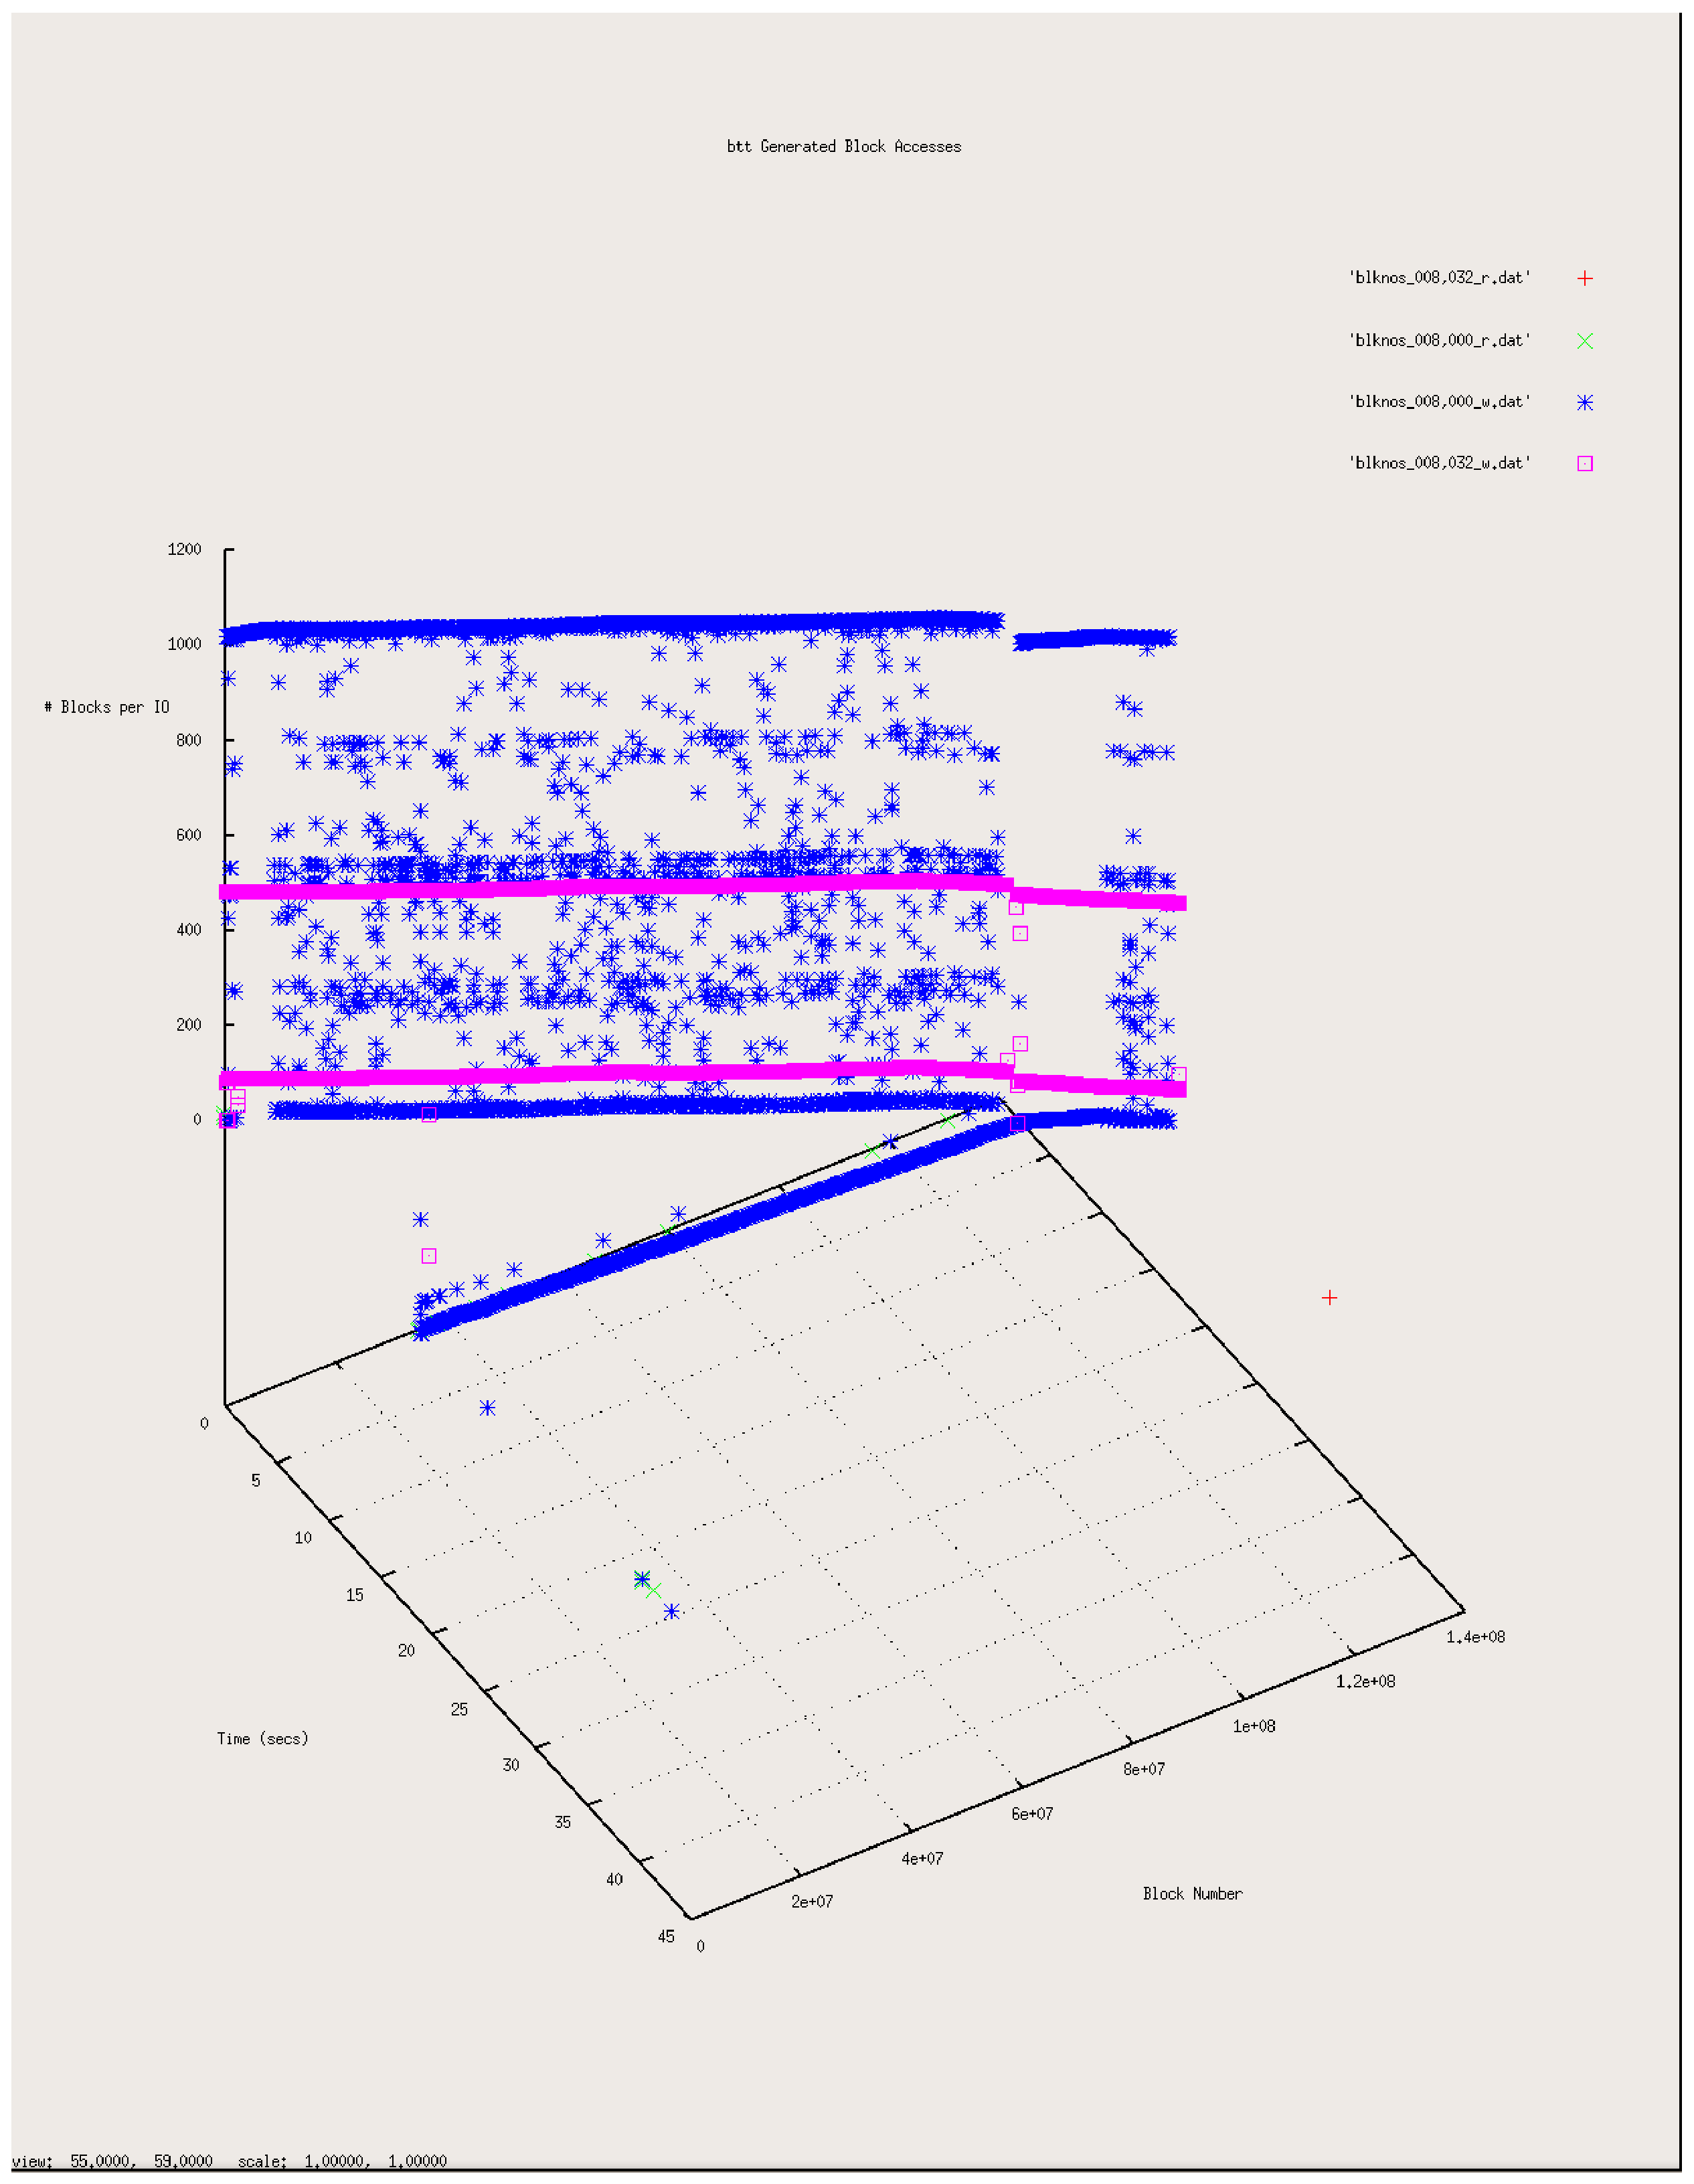
\epsfig{file=bno_plot.eps,width=5.5in}
\caption{\label{fig:bno_plot}Sample \texttt{bno\_plot.py} Screen Shot}
\end{figure}

\clearpage
\newpage\section{\label{sec:appendix}Sample \texttt{btt}
Output}
  Here is a complete output file from a btt run, illustrating a lot of the
  capabilities of btt.
\begin{verbatim}
==================== All Devices ====================

            ALL           MIN           AVG           MAX           N
--------------- ------------- ------------- ------------- -----------
Q2Qdm             0.000001260   0.000078915  14.504199709      491531
Q2Adm             0.000000398   0.001184212  43.228889856      491566

Q2Q               0.000000455   0.000009032   1.811181609      491566
Q2G               0.000000466   0.002396857   0.203392940        8756
G2I               0.000000142   0.000000461   0.000096257        8756
Q2M               0.000000230   0.000000433   0.000173083      482810
I2D               0.000000999   0.407286973   0.982146009        8756
M2D               0.000001251   0.356512650   0.982143260      482810
D2C               0.000057729   0.037337508   2.011319687      491566
Q2C               0.000060550   0.394797701   2.035625308      491566

==================== Device Overhead ====================

       DEV |       Q2G       G2I       Q2M       I2D       D2C
---------- | --------- --------- --------- --------- ---------
 (  8,  0) |   0.3104%   0.0004%   0.0003%  58.9079%  41.0914%
 (  8, 32) |   0.5858%   0.0001%   0.0001%  98.3852%   1.6146%
---------- | --------- --------- --------- --------- ---------
   Overall |   0.0957%   0.0000%   0.0010%  16.2534%  83.6500%

\end{verbatim}
\newpage
\begin{verbatim}

==================== Device Merge Information ====================

       DEV |       #Q       #D   Ratio |   BLKmin   BLKavg   BLKmax    Total
---------- | -------- -------- ------- | -------- -------- -------- --------
 (  8,  0) |   246812     3970    62.2 |        2      497     1024  1974490
 (  8, 32) |   244754     4786    51.1 |        8      409      488  1958032
---------- | -------- -------- ------- | -------- -------- -------- --------
       DEV |       #Q       #D   Ratio |   BLKmin   BLKavg   BLKmax    Total
     TOTAL |   491566     8756    56.1 |        2      449     1024  3932522

==================== Device Q2Q Seek Information ====================

       DEV |          NSEEKS            MEAN          MEDIAN | MODE
---------- | --------------- --------------- --------------- | ---------------
 (  9,  0) |          491532          2693.5               0 | 0(489746)
 (  8,  0) |          246812          2682.4               0 | 0(245021)
 (  8, 32) |          244754          1355.3               0 | 0(243795)
---------- | --------------- --------------- --------------- | ---------------
   Overall |          NSEEKS            MEAN          MEDIAN | MODE
   Average |          983098          2357.6               0 | 0(978562)

==================== Device D2D Seek Information ====================

       DEV |          NSEEKS            MEAN          MEDIAN | MODE
---------- | --------------- --------------- --------------- | ---------------
 (  8,  0) |            3970        219326.9               0 | 0(2177)
 (  8, 32) |            4786         69254.5               0 | 0(3828)
---------- | --------------- --------------- --------------- | ---------------
   Overall |          NSEEKS            MEAN          MEDIAN | MODE
   Average |            8756        137297.8               0 | 0(6005)

\end{verbatim}
\newpage
\begin{verbatim}

==================== Plug Information ====================

       DEV |    # Plugs # Timer Us  | % Time Q Plugged
---------- | ---------- ----------  | ----------------
 (  8,  0) |       1152(       137) |   0.107460846%
 (  8, 32) |          5(         0) |   0.000175916%
---------- | ---------- ----------  | ----------------
   Overall |    # Plugs # Timer Us  | % Time Q Plugged
   Average |        578(        68) |   0.053818381%

==================== Active Requests At Q Information ====================

       DEV |  Avg Reqs @ Q
---------- | -------------
 (  8,  0) |          11.1
 (  8, 32) |         133.0
---------- | -------------
   Overall | Avgs Reqs @ Q
   Average |          71.8

==================== Q2D Histogram ====================

       DEV | <.005 <.010 <.025 <.050 <.075 <.100 <.250 <.500 < 1.0 >=1.0
 --------- | ===== ===== ===== ===== ===== ===== ===== ===== ===== =====
 (  8,  0) |  80.5   3.5   1.0   1.0   0.7   0.6   4.0   5.3   3.4   0.0
 (  8, 32) |   0.3   0.0   0.3   0.2   0.2   0.2   1.7   2.0  95.2   0.0
========== | ===== ===== ===== ===== ===== ===== ===== ===== ===== =====
       AVG |  40.5   1.8   0.6   0.6   0.4   0.4   2.8   3.7  49.1   0.0

\end{verbatim}


\end{document}
\subsection{\label{sec:o-B}\texttt{--dump-blocknos}/\texttt{-B}}
